\documentclass[10pt,a4paper]{article}
\usepackage[a4paper, top=2.0cm, bottom=2.2cm, left=2.2cm, right=2.2cm, headsep=0.6cm]{geometry}
\usepackage{fontspec}
\setmainfont{texgyretermes}[Extension=.otf, UprightFont=*-regular, BoldFont=*-bold, ItalicFont=*-italic, BoldItalicFont=*-bolditalic]
\setsansfont{texgyreheros}[Extension=.otf, UprightFont=*-regular, BoldFont=*-bold, ItalicFont=*-italic, BoldItalicFont=*-bolditalic]
\usepackage{babel}
\babelprovide[import, main]{polish}
\usepackage{microtype}
\usepackage{array, booktabs, longtable, tabularx}
\usepackage[table]{xcolor}
\usepackage{graphicx}
\usepackage{enumitem}
\usepackage{parskip}
\usepackage{fancyhdr}
\usepackage{titlesec}
\usepackage[hidelinks]{hyperref}
\emergencystretch=3em
\setlist{itemsep=2pt, topsep=3pt, leftmargin=1.4em}
\definecolor{L1}{HTML}{2A78D6}\definecolor{L2}{HTML}{EB6834}\definecolor{L3}{HTML}{1BAF7A}
\definecolor{L4}{HTML}{EDA100}\definecolor{L7}{HTML}{E87BA4}\definecolor{muted}{HTML}{767A84}
\definecolor{bad}{HTML}{C23030}\definecolor{good}{HTML}{0A8A0A}
\newcommand{\linedot}[1]{\textcolor{#1}{\rule[0.1ex]{0.9ex}{0.9ex}}\,}
\newcommand{\mut}[1]{\textcolor{muted}{#1}}
\titleformat{\section}{\sffamily\large\bfseries}{\thesection.}{0.5em}{}
\titleformat{\subsection}{\sffamily\normalsize\bfseries}{\thesubsection.}{0.5em}{}
\titlespacing*{\section}{0pt}{1.2em}{0.4em}
\titlespacing*{\subsection}{0pt}{0.9em}{0.3em}
\setlength{\LTpre}{4pt}\setlength{\LTpost}{4pt}
\pagestyle{fancy}\fancyhf{}
\renewcommand{\headrulewidth}{0.3pt}
\fancyhead[L]{\sffamily\footnotesize 14-200.pl/@yasiu/2026-09-30-raport-zkm}
\fancyhead[R]{\sffamily\footnotesize Korekty rozkładu ZKM Iława}
\fancyfoot[C]{\sffamily\footnotesize \thepage}
\begin{document}
{\sffamily\footnotesize\bfseries\MakeUppercase{Raport ZKM Iława · propozycja korekt}}\par\smallskip
{\sffamily\LARGE\bfseries Korekty rozkładu ZKM Iława}\par\medskip
{\large Przesunięcia kursów o kilka minut, które dają więcej przesiadek z pociągów i do pociągów na przystanku Dworcowa.}\par\medskip
{\small\mut{Rozkład ZKM ważny od 1.09.2026. Przystanki: 005-01, 079-00. Obliczenia z dnia 30.09.2026.}}\par\bigskip
\section*{Wynik}
Obiegi autobusów, przerwy kierowców, liczba autobusów i łączny czas pracy kierowców zostają zachowane. Przesiadka jest dobra, gdy po dojściu z peronu (4 min) lub na peron (5 min) czeka się najwyżej 5 min. Liczone są pary pociąg--linia, bo podróżny potrzebuje konkretnej linii. Narzędzie usuwa też „uciekające” odjazdy: autobus nie powinien odjeżdżać tuż przed dojściem podróżnych, gdy następny kurs linii jest dużo później. Autobus może tylko przyjechać na Dworcową wcześniej albo odjechać z niej później, więc każda zmiana daje przesiadce więcej czasu. Wyniki dotyczą wariantu: obiegi jednej linii.
{\footnotesize
\begin{center}\begin{tabular}{@{}p{5.4cm} r r r@{}}\toprule
Wskaźnik & Dzień & Sobota & Niedziela \\ \midrule
Dobre przesiadki dziennie (czekanie do 5 min) & 84 → 130 \mut{(+56\,\%)} & 45 → 63 \mut{(+40\,\%)} & 27 → 35 \mut{(+29\,\%)} \\
Przesiadki z czekaniem do 10 min dziennie & 155 → 201 \mut{(+30\,\%)} & 91 → 108 \mut{(+19\,\%)} & 49 → 57 \mut{(+18\,\%)} \\
„Uciekające” odjazdy: pary pociąg--linia dziennie & 34 → 13 \mut{($-$62\,\%)} & 26 → 15 \mut{($-$42\,\%)} & 14 → 10 \mut{($-$29\,\%)} \\
Zmienione kursy (wszystkie etapy) & 51 z 188 & 19 z 89 & 9 z 54 \\
Godziny pracy kierowców dziennie & 197,4 → 196,7 & 69,8 → 69,6 & 53,5 → 53,3 \\
Autobusy w szczycie & 18 → 18 & 6 → 6 & 5 → 5 \\
Służby z przerwą zgodną z ustawą & 34/34 → 34/34 & 11/11 → 11/11 & 10/10 → 10/10 \\
\bottomrule\end{tabular}\end{center}}
\section{Etapy wdrożenia}
Każdy etap zachowuje zmiany poprzedniego i dodaje kolejne, więc rozkład można zmieniać krok po kroku. Etap 1 to 20 najbardziej opłacalnych zmian, etap 2 to łącznie 40 zmian, ostatni etap nie ma limitu.
\par\medskip\noindent\begin{minipage}{\textwidth}\centering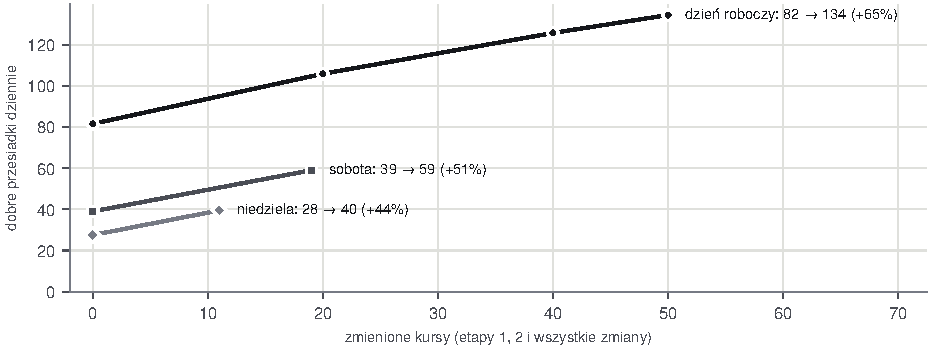
\includegraphics[width=\textwidth]{fig/korekty-etapy.pdf}\par\smallskip
{\small\mut{Rys. 1. Dobre przesiadki dziennie po kolejnych etapach.}}\end{minipage}\par\medskip
{\small
\begin{center}\begin{tabular}{@{}l l r r r r@{}}\toprule
Dzień & Etap & Zmienione kursy & Dobre przesiadki/dzień & Zmiana & Do 10 min/dzień \\ \midrule
dzień roboczy & obecny rozkład & 0 & 84 & -- & 155 \\
 & etap 1 & 20 & 103 & +23\,\% & 178 \\
 & etap 2 & 40 & 123 & +47\,\% & 197 \\
 & etap 3 & 51 & 130 & +56\,\% & 201 \\
sobota & obecny rozkład & 0 & 45 & -- & 91 \\
 & etap 1 & 19 & 63 & +40\,\% & 108 \\
niedziela & obecny rozkład & 0 & 27 & -- & 49 \\
 & etap 1 & 9 & 35 & +29\,\% & 57 \\
\bottomrule\end{tabular}\end{center}}
Pełny wykaz zmienionych kursów, z pociągami, dla których przesiadka staje się dogodna, jest w ostatnim rozdziale.
\section{Odjazdy, które „uciekają” pociągom}
Odjazd „ucieka”, gdy autobus odjeżdża od 2 min przed przyjazdem pociągu do chwili, w której podróżni dochodzą na przystanek, a następny kurs tej linii jest za 30 min lub później. Korekta usuwa większość takich przypadków prostym przesunięciem kursu. Pozostałe wymagają zmian, które musi ocenić ZKM: przesunięcia o więcej niż kilka minut, zmiany obiegu autobusu albo służby kierowcy. Na dni z dużymi opóźnieniami pociągów odpowiedzią może być linia przesiadkowa.
{\footnotesize
\begin{center}\begin{tabular}{@{}l r r r r r@{}}\toprule
Typ dnia & Pary dziennie: obecnie & po korekcie & Zmiana & Rozwiązane w dniu planowania & Do decyzji ZKM \\ \midrule
Dzień roboczy & 34,1 & 12,8 & $-$62\,\% & 25 z 34 & 12 \\
Sobota & 26,0 & 15,0 & $-$42\,\% & 14 z 26 & 15 \\
Niedziela i święta & 13,8 & 9,8 & $-$29\,\% & 4 z 14 & 10 \\
\bottomrule\end{tabular}\end{center}}
\subsection*{Dzień roboczy (1.10.2026)}
{\footnotesize
\begin{longtable}{@{}l l l l p{7.4cm}@{}}\toprule
Odjazd & Linia & Następny & Po korekcie & Pociągi i wynik \\ \midrule\endhead
\bottomrule\endfoot
6:42 & \linedot{L1}1 & 7:24 & 6:44 & 06:39 IC 5708: rozwiązane; 06:44 R 90101: ZKM \\
6:52 & \linedot{L3}3 & 7:30 & 6:54 & 06:50 R 90623: rozwiązane; 06:52 EIP 5300: ZKM \\
7:00 & \linedot{L2}2 & 7:30 & 7:04 & 06:59 TLK 35171: rozwiązane; 06:59 TLK 53104: rozwiązane \\
7:24 & \linedot{L1}1 & 8:00 & 7:26 & 07:22 R 90240: rozwiązane \\
8:40 & \linedot{L2}2 & 9:30 & bez zmiany & 08:39 IC 1618: ZKM \\
8:40 & \linedot{L4}4 & 9:45 & bez zmiany & 08:39 IC 1618: ZKM \\
9:03 & \linedot{L3}3 & 9:41 & 9:07 & 09:02 EIP 1503: rozwiązane \\
9:15 & \linedot{L7}7 & 15:50 & bez zmiany & 09:16 IC 7503: ZKM \\
10:55 & \linedot{L3}3 & 11:50 & 11:00 & 10:52 EIP 5402: rozwiązane; 10:55 IC 1513: rozwiązane \\
11:20 & \linedot{L4}4 & 12:23 & 11:21 & 11:16 IC 6115: rozwiązane \\
11:50 & \linedot{L3}3 & 12:29 & 11:52 & 11:48 R 90654: rozwiązane \\
12:53 & \linedot{L3}3 & 13:28 & bez zmiany & 12:52 EIP 5352: ZKM \\
13:00 & \linedot{L2}2 & 13:35 & 13:03 & 12:58 IC 1815: rozwiązane; 12:58 IC 5114: rozwiązane \\
14:35 & \linedot{L2}2 & 15:07 & 14:38 & 14:33 IC 5714: rozwiązane \\
15:02 & \linedot{L1}1 & 16:35 & bez zmiany & 15:02 EIP 3553: ZKM \\
15:40 & \linedot{L3}3 & 16:10 & 15:42 & 15:38 R 90244: rozwiązane \\
16:35 & \linedot{L1}1 & 17:55 & 16:40 & 16:34 R 90625: rozwiązane; 16:35 IC 1614: rozwiązane \\
16:45 & \linedot{L3}3 & 17:15 & 16:49 & 16:45 R 90656: rozwiązane \\
17:55 & \linedot{L1}1 & 19:55 & 17:57 & 17:52 EIP 5406: rozwiązane \\
18:38 & \linedot{L2}2 & 19:08 & bez zmiany & 18:39 IC 5702: ZKM \\
19:55 & \linedot{L1}1 & 21:04 & 19:57 & 19:52 EIP 5102: rozwiązane \\
20:06 & \linedot{L2}2 & 20:46 & 20:08 & 20:04 IC 5320: rozwiązane \\
21:04 & \linedot{L1}1 & brak & 21:07 & 21:02 EIP 3503: rozwiązane; 21:03 R 90113: rozwiązane; 21:06 TLK 53170: ZKM \\
21:06 & \linedot{L2}2 & 22:20 & 21:10 & 21:02 EIP 3503: rozwiązane; 21:03 R 90113: rozwiązane; 21:06 TLK 53170: rozwiązane \\
\end{longtable}}
Przypadki do decyzji ZKM (po korekcie):
{\footnotesize
\begin{longtable}{@{}l l l l p{6.4cm}@{}}\toprule
Odjazd & Linia & Pociąg & Następny & Co jest potrzebne \\ \midrule\endhead
\bottomrule\endfoot
6:44 & \linedot{L1}1 & 06:44 R 90101 & 7:26 & potrzebne przesunięcie o 6 min, większe niż 5 min: zmiana rozkładu linii lub obiegu \\
6:54 & \linedot{L3}3 & 06:52 EIP 5300 & 7:30 & przesunięcie możliwe, ale kosztem innych przesiadek albo nowego „uciekającego” odjazdu \\
8:40 & \linedot{L2}2 & 08:39 IC 1618 & 9:30 & przesunięcie możliwe, ale kosztem innych przesiadek albo nowego „uciekającego” odjazdu \\
8:40 & \linedot{L4}4 & 08:39 IC 1618 & 9:45 & przesunięcie możliwe, ale kosztem innych przesiadek albo nowego „uciekającego” odjazdu \\
9:15 & \linedot{L7}7 & 09:16 IC 7503 & 15:50 & potrzebne przesunięcie o 6 min, większe niż 5 min: zmiana rozkładu linii lub obiegu \\
11:52 & \linedot{L3}3 & 11:52 EIP 5302 (nowy) & 12:29 & potrzebne przesunięcie o 7 min, większe niż 5 min: zmiana rozkładu linii lub obiegu \\
12:53 & \linedot{L3}3 & 12:52 EIP 5352 & 13:28 & przesunięcie możliwe, ale kosztem innych przesiadek albo nowego „uciekającego” odjazdu \\
13:03 & \linedot{L2}2 & 13:02 EIP 4507 (nowy) & 13:35 & potrzebne przesunięcie o 7 min, większe niż 5 min: zmiana rozkładu linii lub obiegu \\
15:02 & \linedot{L1}1 & 15:02 EIP 3553 & 16:40 & autobus nie ma zapasu postoju przed kolejnym kursem albo kierowca straciłby przerwę: zmiana obiegu lub służby \\
16:40 & \linedot{L1}1 & 16:38 R 90225 (nowy) & 17:57 & potrzebne przesunięcie o 7 min, większe niż 5 min: zmiana rozkładu linii lub obiegu \\
18:38 & \linedot{L2}2 & 18:39 IC 5702 & 19:08 & potrzebne przesunięcie o 6 min, większe niż 5 min: zmiana rozkładu linii lub obiegu \\
21:07 & \linedot{L1}1 & 21:06 TLK 53170 & brak & potrzebne przesunięcie o 6 min, większe niż 5 min: zmiana rozkładu linii lub obiegu \\
\end{longtable}}
\subsection*{Sobota (3.10.2026)}
{\footnotesize
\begin{longtable}{@{}l l l l p{7.4cm}@{}}\toprule
Odjazd & Linia & Następny & Po korekcie & Pociągi i wynik \\ \midrule\endhead
\bottomrule\endfoot
5:42 & \linedot{L2}2 & 6:15 & bez zmiany & 05:40 R 90621: ZKM; 05:44 R 90205: ZKM \\
6:50 & \linedot{L1}1 & 8:10 & bez zmiany & 06:50 R 90623: ZKM \\
7:54 & \linedot{L3}3 & 8:26 & 7:59 & 07:55 IC 1521: rozwiązane \\
9:00 & \linedot{L3}3 & 9:45 & 9:03 & 08:57 IC 1857: rozwiązane; 08:58 IC 5116: rozwiązane \\
9:05 & \linedot{L1}1 & 10:05 & 9:07 & 09:02 EIP 1503: rozwiązane \\
11:10 & \linedot{L2}2 & 12:01 & bez zmiany & 11:12 TLK 8328: ZKM \\
11:52 & \linedot{L3}3 & 12:35 & bez zmiany & 11:52 EIP 5302: ZKM \\
12:01 & \linedot{L2}2 & 13:01 & bez zmiany & 12:02 EIP 3509: ZKM \\
13:01 & \linedot{L2}2 & 14:11 & 13:02 & 12:58 IC 1815: rozwiązane; 12:58 IC 5114: rozwiązane; 13:02 EIP 4507: ZKM \\
13:20 & \linedot{L1}1 & 15:00 & 13:21 & 13:16 IC 7515: rozwiązane \\
14:05 & \linedot{L3}3 & 14:35 & 14:07 & 14:02 EIP 3507: rozwiązane \\
14:35 & \linedot{L3}3 & 15:33 & 14:38 & 14:33 IC 5714: rozwiązane \\
15:00 & \linedot{L1}1 & brak & 15:02 & 14:57 IC 1515: rozwiązane; 14:58 IC 8114: rozwiązane \\
16:37 & \linedot{L2}2 & 18:10 & 16:38 & 16:34 R 90625: rozwiązane; 16:35 IC 1614: ZKM; 16:38 R 90225: ZKM \\
17:21 & \linedot{L3}3 & 19:15 & bez zmiany & 17:21 IC 7511: ZKM \\
19:15 & \linedot{L3}3 & 21:06 & bez zmiany & 19:16 IC 6119: ZKM \\
21:06 & \linedot{L3}3 & brak & 21:07 & 21:02 EIP 3503: rozwiązane; 21:03 R 90113: rozwiązane; 21:06 TLK 53170: ZKM \\
\end{longtable}}
Przypadki do decyzji ZKM (po korekcie):
{\footnotesize
\begin{longtable}{@{}l l l l p{6.4cm}@{}}\toprule
Odjazd & Linia & Pociąg & Następny & Co jest potrzebne \\ \midrule\endhead
\bottomrule\endfoot
5:42 & \linedot{L2}2 & 05:40 R 90621 & 6:15 & autobus nie ma zapasu postoju przed kolejnym kursem albo kierowca straciłby przerwę: zmiana obiegu lub służby \\
5:42 & \linedot{L2}2 & 05:44 R 90205 & 6:15 & potrzebne przesunięcie o 6 min, większe niż 5 min: zmiana rozkładu linii lub obiegu \\
6:50 & \linedot{L1}1 & 06:50 R 90623 & 8:10 & autobus nie ma zapasu postoju przed kolejnym kursem albo kierowca straciłby przerwę: zmiana obiegu lub służby \\
9:03 & \linedot{L3}3 & 09:02 EIP 1503 (nowy) & 9:45 & potrzebne przesunięcie o 7 min, większe niż 5 min: zmiana rozkładu linii lub obiegu \\
11:10 & \linedot{L2}2 & 11:12 TLK 8328 & 12:01 & potrzebne przesunięcie o 6 min, większe niż 5 min: zmiana rozkładu linii lub obiegu \\
11:52 & \linedot{L3}3 & 11:52 EIP 5302 & 12:35 & autobus nie ma zapasu postoju przed kolejnym kursem albo kierowca straciłby przerwę: zmiana obiegu lub służby \\
12:01 & \linedot{L2}2 & 12:02 EIP 3509 & 13:02 & potrzebne przesunięcie o 6 min, większe niż 5 min: zmiana rozkładu linii lub obiegu \\
13:02 & \linedot{L2}2 & 13:02 EIP 4507 & 14:11 & potrzebne przesunięcie o 6 min, większe niż 5 min: zmiana rozkładu linii lub obiegu \\
14:38 & \linedot{L3}3 & 14:38 R 55205 (nowy) & 15:33 & potrzebne przesunięcie o 7 min, większe niż 5 min: zmiana rozkładu linii lub obiegu \\
15:02 & \linedot{L1}1 & 15:02 EIP 3553 (nowy) & brak & potrzebne przesunięcie o 7 min, większe niż 5 min: zmiana rozkładu linii lub obiegu \\
16:38 & \linedot{L2}2 & 16:35 IC 1614 & 18:10 & autobus nie ma zapasu postoju przed kolejnym kursem albo kierowca straciłby przerwę: zmiana obiegu lub służby \\
16:38 & \linedot{L2}2 & 16:38 R 90225 & 18:10 & autobus nie ma zapasu postoju przed kolejnym kursem albo kierowca straciłby przerwę: zmiana obiegu lub służby \\
17:21 & \linedot{L3}3 & 17:21 IC 7511 & 19:15 & autobus nie ma zapasu postoju przed kolejnym kursem albo kierowca straciłby przerwę: zmiana obiegu lub służby \\
19:15 & \linedot{L3}3 & 19:16 IC 6119 & 21:07 & potrzebne przesunięcie o 6 min, większe niż 5 min: zmiana rozkładu linii lub obiegu \\
21:07 & \linedot{L3}3 & 21:06 TLK 53170 & brak & autobus nie ma zapasu postoju przed kolejnym kursem albo kierowca straciłby przerwę: zmiana obiegu lub służby \\
\end{longtable}}
\subsection*{Niedziela i święta (4.10.2026)}
{\footnotesize
\begin{longtable}{@{}l l l l p{7.4cm}@{}}\toprule
Odjazd & Linia & Następny & Po korekcie & Pociągi i wynik \\ \midrule\endhead
\bottomrule\endfoot
7:58 & \linedot{L3}3 & 9:16 & 7:59 & 07:55 IC 1521: rozwiązane \\
9:00 & \linedot{L2}2 & 10:51 & bez zmiany & 08:57 IC 1553: ZKM; 08:58 IC 5116: ZKM \\
9:16 & \linedot{L3}3 & 10:00 & bez zmiany & 09:16 IC 7503: ZKM \\
10:51 & \linedot{L2}2 & 12:52 & bez zmiany & 10:52 EIP 5402: ZKM \\
10:58 & \linedot{L1}1 & 12:47 & 11:00 & 10:55 IC 1513: rozwiązane \\
11:46 & \linedot{L3}3 & 12:20 & bez zmiany & 11:48 R 90654: ZKM \\
12:52 & \linedot{L2}2 & 14:38 & bez zmiany & 12:52 EIP 5352: ZKM \\
14:38 & \linedot{L2}2 & 16:32 & 14:42 & 14:38 R 55205: rozwiązane \\
15:40 & \linedot{L1}1 & brak & 15:42 & 15:38 R 90244: rozwiązane \\
16:32 & \linedot{L2}2 & 18:10 & bez zmiany & 16:34 R 90625: ZKM \\
17:21 & \linedot{L3}3 & 19:15 & bez zmiany & 17:21 IC 7511: ZKM \\
19:15 & \linedot{L3}3 & 21:08 & bez zmiany & 19:16 IC 6119: ZKM \\
21:08 & \linedot{L3}3 & brak & bez zmiany & 21:06 TLK 53170: ZKM \\
\end{longtable}}
Przypadki do decyzji ZKM (po korekcie):
{\footnotesize
\begin{longtable}{@{}l l l l p{6.4cm}@{}}\toprule
Odjazd & Linia & Pociąg & Następny & Co jest potrzebne \\ \midrule\endhead
\bottomrule\endfoot
9:00 & \linedot{L2}2 & 08:57 IC 1553 & 10:51 & przesunięcie możliwe, ale kosztem innych przesiadek albo nowego „uciekającego” odjazdu \\
9:00 & \linedot{L2}2 & 08:58 IC 5116 & 10:51 & autobus nie ma zapasu postoju przed kolejnym kursem albo kierowca straciłby przerwę: zmiana obiegu lub służby \\
9:16 & \linedot{L3}3 & 09:16 IC 7503 & 10:00 & autobus nie ma zapasu postoju przed kolejnym kursem albo kierowca straciłby przerwę: zmiana obiegu lub służby \\
10:51 & \linedot{L2}2 & 10:52 EIP 5402 & 12:52 & potrzebne przesunięcie o 6 min, większe niż 5 min: zmiana rozkładu linii lub obiegu \\
11:46 & \linedot{L3}3 & 11:48 R 90654 & 12:20 & potrzebne przesunięcie o 6 min, większe niż 5 min: zmiana rozkładu linii lub obiegu \\
12:52 & \linedot{L2}2 & 12:52 EIP 5352 & 14:42 & przesunięcie możliwe, ale kosztem innych przesiadek albo nowego „uciekającego” odjazdu \\
16:32 & \linedot{L2}2 & 16:34 R 90625 & 18:10 & potrzebne przesunięcie o 6 min, większe niż 5 min: zmiana rozkładu linii lub obiegu \\
17:21 & \linedot{L3}3 & 17:21 IC 7511 & 19:15 & autobus nie ma zapasu postoju przed kolejnym kursem albo kierowca straciłby przerwę: zmiana obiegu lub służby \\
19:15 & \linedot{L3}3 & 19:16 IC 6119 & 21:08 & potrzebne przesunięcie o 6 min, większe niż 5 min: zmiana rozkładu linii lub obiegu \\
21:08 & \linedot{L3}3 & 21:06 TLK 53170 & brak & autobus nie ma zapasu postoju przed kolejnym kursem albo kierowca straciłby przerwę: zmiana obiegu lub służby \\
\end{longtable}}
\section{Test na minionych dniach}
Obecny rozkład, etapy i pełną propozycję sprawdzono na 19 minionych dniach z danymi o opóźnieniach (11.09.2026--29.09.2026). Rozkład ZKM i planowy rozkład pociągów są te same, zmieniają się tylko rzeczywiste godziny pociągów. „Dobre”: czekanie po dojściu do 5 min. Wartości to średnie na dzień. Nowszy pomiar faktycznych przyjazdów (monitor PKP PLK, wszyscy przewoźnicy, także październik) jest w raporcie „Przesiadki Iława Główna”.

{\footnotesize
\begin{center}\begin{tabular}{@{}l l r r r r@{}}\toprule
Dzień & Rozkład & Dni & Dobre: plan & rzecz. & Czekanie po pociągu [min] \\ \midrule
dzień roboczy & obecny rozkład & 13 & 83 & 86 & 37,0 \\
 & etap 1 & 13 & 103 & 99 & 35,5 \\
 & etap 2 & 13 & 124 & 116 & 35,4 \\
 & pełna propozycja & 13 & 131 & 120 & 35,4 \\
sobota & obecny rozkład & 3 & 45 & 44 & 39,0 \\
 & etap 1 & 3 & 63 & 57 & 37,3 \\
 & etap 2 & 3 & 63 & 57 & 37,3 \\
 & pełna propozycja & 3 & 63 & 57 & 37,3 \\
niedziela & obecny rozkład & 3 & 27 & 27 & 45,5 \\
 & etap 1 & 3 & 35 & 33 & 44,7 \\
 & etap 2 & 3 & 35 & 33 & 44,7 \\
 & pełna propozycja & 3 & 35 & 33 & 44,7 \\
\bottomrule\end{tabular}\end{center}}
Najgorsze dni (najwięcej pociągów spóźnionych ponad 5 min):
\begin{itemize}
\item dzień roboczy 28.09.2026: 24 pociągi spóźnionych ponad 5 min, średnie opóźnienie 12,0 min; dobre przesiadki 90 $\to$ 105.
\item sobota 26.09.2026: 13 pociągów spóźnionych ponad 5 min, średnie opóźnienie 2,8 min; dobre przesiadki 41 $\to$ 51.
\item niedziela 27.09.2026: 25 pociągów spóźnionych ponad 5 min, średnie opóźnienie 21,7 min; dobre przesiadki 24 $\to$ 27.
\end{itemize}
\mut{\footnotesize Czekanie po pociągu: średni czas od dojścia na przystanek do odjazdu najbliższego autobusu danej linii, dla wszystkich par pociąg--linia, najwyżej 60 min. W 16 z 19 dni rzeczywiste godziny są znane tylko dla części pociągów (głównie PKP Intercity); pozostałe pociągi liczą się jako punktualne.}
\section{Odjazdy z przystanku Dworcowa po korekcie}
Godziny odjazdów w dniu planowania. Zmienione godziny: obecna $\to$ \textbf{proponowana}.
\subsection*{Dzień roboczy (1.10.2026)}
{\footnotesize
\noindent\linedot{L1}1\textbf{Linia 1:} 5:05, 6:42$\to$\textbf{6:44}, 7:24$\to$\textbf{7:26}, 8:00, 8:35, 10:05, 11:25, 12:40$\to$\textbf{12:44}, 13:08, 13:30, 14:35$\to$\textbf{14:38}, 15:02, 16:35$\to$\textbf{16:40}, 17:55$\to$\textbf{17:57}, 19:55$\to$\textbf{19:57}, 21:04$\to$\textbf{21:07}\par\smallskip
\noindent\linedot{L2}2\textbf{Linia 2:} 5:38, 6:05, 6:36, 7:00$\to$\textbf{7:04}, 7:30, 8:08, 8:40, 9:30, 9:50, 10:23, 11:04, 11:30, 12:10, 13:00$\to$\textbf{13:03}, 13:35, 14:25, 14:35$\to$\textbf{14:38}, 15:07, 15:30, 15:45, 16:25$\to$\textbf{16:30}, 16:50, 17:46, 18:38, 19:08, 19:23, 20:06$\to$\textbf{20:08}, 20:46, 21:06$\to$\textbf{21:10}, 22:20\par\smallskip
\noindent\linedot{L3}3\textbf{Linia 3:} 5:10, 5:52, 6:20, 6:45$\to$\textbf{6:48}, 6:52$\to$\textbf{6:54}, 7:30, 7:45, 7:52, 8:34, 9:03$\to$\textbf{9:07}, 9:41, 10:36, 10:55$\to$\textbf{11:00}, 11:50$\to$\textbf{11:52}, 12:29, 12:36, 12:53, 13:28, 13:30, 13:38, 13:50, 14:30, 14:48, 15:16, 15:20$\to$\textbf{15:21}, 15:40$\to$\textbf{15:42}, 16:10, 16:45$\to$\textbf{16:49}, 17:15, 18:08, 18:24, 19:27, 19:57, 20:42, 21:38, 22:15\par\smallskip
\noindent\linedot{L4}4\textbf{Linia 4:} 7:30, 8:40, 9:45, 11:20$\to$\textbf{11:21}, 12:23, 13:40, 15:10\par\smallskip
\noindent\linedot{L7}7\textbf{Linia 7:} 9:15, 15:50\par\smallskip
}
\subsection*{Sobota (3.10.2026)}
{\footnotesize
\noindent\linedot{L1}1\textbf{Linia 1:} 6:50, 8:10, 9:05$\to$\textbf{9:07}, 10:05, 11:45, 13:20$\to$\textbf{13:21}, 15:00$\to$\textbf{15:02}\par\smallskip
\noindent\linedot{L2}2\textbf{Linia 2:} 5:42, 6:15, 6:35, 7:11, 7:40, 8:32, 9:25, 10:20, 11:10, 12:01, 13:01$\to$\textbf{13:02}, 14:11, 15:10, 16:37$\to$\textbf{16:38}, 18:10, 20:17\par\smallskip
\noindent\linedot{L3}3\textbf{Linia 3:} 5:22, 6:02, 6:29, 7:04, 7:36, 7:54$\to$\textbf{7:59}, 8:26, 9:00$\to$\textbf{9:03}, 9:45, 10:35, 10:45, 11:30, 11:52, 12:35, 13:35, 14:05$\to$\textbf{14:07}, 14:35$\to$\textbf{14:38}, 15:33, 17:21, 19:15, 21:06$\to$\textbf{21:07}\par\smallskip
}
\subsection*{Niedziela i święta (4.10.2026)}
{\footnotesize
\noindent\linedot{L1}1\textbf{Linia 1:} 8:15, 9:35, 10:58$\to$\textbf{11:00}, 12:47, 14:15, 15:40$\to$\textbf{15:42}\par\smallskip
\noindent\linedot{L2}2\textbf{Linia 2:} 7:07, 9:00, 10:51, 12:52, 14:38$\to$\textbf{14:42}, 16:32, 18:10, 20:17\par\smallskip
\noindent\linedot{L3}3\textbf{Linia 3:} 6:05, 7:58$\to$\textbf{7:59}, 9:16, 10:00, 11:00, 11:46, 12:20, 13:46, 14:30, 15:35, 17:21, 19:15, 21:08\par\smallskip
}
\section{Obiegi autobusów i służby kierowców}
Każdy wiersz to jeden autobus, każdy pasek to kurs. Obiegi odtworzono z rozkładu, bo ZKM ich nie publikuje: autobus bierze najbliższy kurs z tego samego przystanku końcowego, najpierw tej samej linii. Przesunięcia mieszczą się w postojach, więc obiegi się nie zmieniają.
\par\medskip\noindent\begin{minipage}{\textwidth}\centering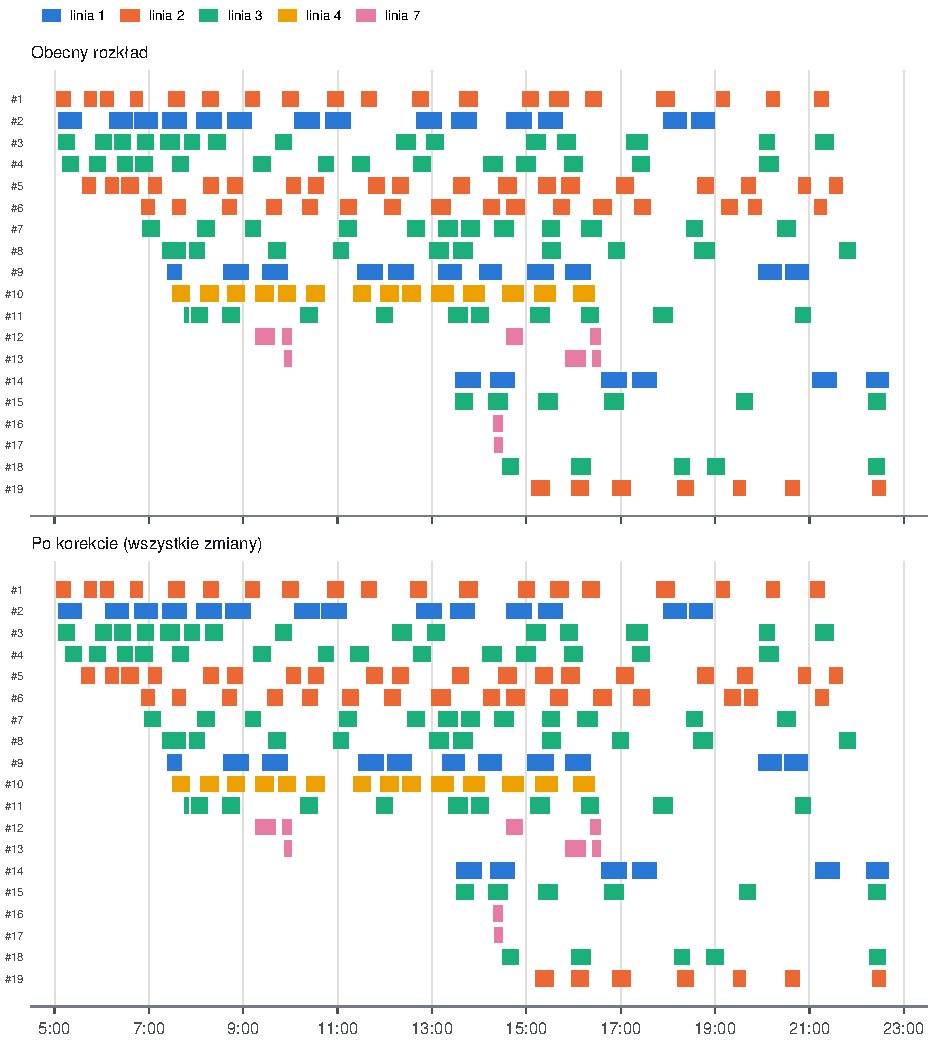
\includegraphics[width=\textwidth]{fig/korekty-obiegi.pdf}\par\smallskip
{\small\mut{Rys. 2. Obiegi autobusów w dzień roboczy (obiegi jednej linii).}}\end{minipage}\par\medskip
Obiegi podzielono na służby kierowców na Dworcowej (najdłużej 8,5 godz. z przygotowaniem). Przerwa: przy ponad 6 godz. jazdy co najmniej 30 min, przy ponad 8 godz. 45 min, w częściach po co najmniej 15 min w rozkładzie. Zgodnych służb w dzień roboczy: 34 z 34 obecnie, 34 z 34 po korekcie.
{\footnotesize
\begin{longtable}{@{}l l l r p{5.2cm} r l@{}}\toprule
Autobus & Od & Do & Jazda [h] & Przerwy [min] & Wymagane &  \\ \midrule\endhead
\bottomrule\endfoot
\#1 & 04:48 & 12:54 & 3,6 & 17, 20, 32, 22, 34, 28, 36, 22, 43 & -- & zgodna \\
\#1 & 13:20 & 21:20 & 2,8 & 51, 18, 18, 72, 52, 48, 37 & -- & zgodna \\
\#2 & 04:50 & 11:12 & 4,2 & 30, 55 & -- & zgodna \\
\#2 & 12:29 & 19:00 & 3,2 & 43, 130 & -- & zgodna \\
\#3 & 04:50 & 12:35 & 3,4 & 25, 66, 127 & -- & zgodna \\
\#3 & 12:38 & 17:35 & 1,6 & 104, 17, 63 & -- & zgodna \\
\#3 & 19:42 & 21:32 & 0,7 & 51 & -- & zgodna \\
\#4 & 04:55 & 11:40 & 2,9 & 24, 82, 60, 21 & -- & zgodna \\
\#4 & 12:21 & 20:22 & 2,4 & 65, 19, 35, 62, 139 & -- & zgodna \\
\#5 & 05:19 & 13:48 & 3,6 & 16, 49, 55, 54, 55 & -- & zgodna \\
\#5 & 14:10 & 21:43 & 2,8 & 23, 47, 81, 30, 58, 22 & -- & zgodna \\
\#6 & 06:35 & 14:27 & 3,1 & 22, 46, 38, 25, 28, 35, 42, 38 & -- & zgodna \\
\#6 & 14:23 & 21:27 & 2,5 & 29, 37, 22, 90, 75 & -- & zgodna \\
\#7 & 06:39 & 14:45 & 3,1 & 46, 42, 95, 64, 16, 19 & -- & zgodna \\
\#7 & 15:06 & 20:43 & 1,6 & 21, 113, 95 & -- & zgodna \\
\#8 & 07:02 & 13:22 & 2,0 & 80, 65, 97 & -- & zgodna \\
\#8 & 13:13 & 18:58 & 1,6 & 88, 65, 82 & -- & zgodna \\
\#8 & 21:23 & 22:00 & 0,4 & -- & -- & zgodna \\
\#9 & 07:11 & 14:29 & 3,5 & 45, 17, 88, 33, 21 & -- & zgodna \\
\#9 & 14:47 & 21:00 & 2,1 & 15, 215 & -- & zgodna \\
\#10 & 07:15 & 14:54 & 4,9 & 37, 18 & -- & zgodna \\
\#10 & 14:55 & 16:28 & 0,9 & 22 & -- & zgodna \\
\#11 & 07:30 & 15:31 & 2,8 & 18, 77, 76, 68, 52 & -- & zgodna \\
\#11 & 15:55 & 21:03 & 1,2 & 69, 155 & -- & zgodna \\
\#12 & 09:00 & 16:35 & 1,2 & 269, 86 & -- & zgodna \\
\#13 & 09:37 & 16:35 & 0,8 & 343 & -- & zgodna \\
\#14 & 13:15 & 17:47 & 2,2 & 114 & -- & zgodna \\
\#14 & 20:52 & 22:42 & 1,0 & 34 & -- & zgodna \\
\#15 & 13:15 & 17:02 & 1,6 & 19, 39, 57 & -- & zgodna \\
\#15 & 19:12 & 22:38 & 0,8 & 146 & -- & zgodna \\
\#16 & 14:03 & 14:31 & 0,2 & -- & -- & zgodna \\
\#17 & 14:05 & 14:31 & 0,2 & -- & -- & zgodna \\
\#18 & 14:15 & 22:37 & 1,9 & 66, 106, 20, 183 & -- & zgodna \\
\#19 & 14:52 & 22:38 & 2,4 & 27, 30, 58, 49, 49, 92 & -- & zgodna \\
\end{longtable}}
\section{Dodatkowe kursy bez dodatkowego autobusu}
Autobusy, które czekają na Dworcowej dłużej niż jeden kurs tam i z powrotem, mogą wykonać dodatkowy kurs tej samej linii bez nowego autobusu. Gdy postój wypada w środku służby, kierowca jest już w pracy, a kurs przechodzi tylko wtedy, gdy zostaje przerwa wymagana ustawą. Gdy służba kończy się na początku postoju, kurs wydłuża ją o podany czas. Każdy kurs sprawdzono osobno.
{\footnotesize
\begin{longtable}{@{}l l l l l r r r l@{}}\toprule
Dzień & Linia & Odjazd & Powrót & Postój & Nowe dobre & Luka w linii & km & Kierowca \\ \midrule\endhead
\bottomrule\endfoot
dzień roboczy & \linedot{L3}3 & 19:06 & 20:58 & 18:58--21:38 & +4 & 63 min & 13,0 & +2,0 godz. \\
dzień roboczy & \linedot{L2}2 & 17:42 & 18:58 & 17:38--19:08 & +3 & 56 min & 15,3 & w służbie \\
dzień roboczy & \linedot{L1}1 & 15:21 & 16:32 & 14:46--16:40 & +3 & 98 min & 20,7 & w służbie \\
dzień roboczy & \linedot{L1}1 & 19:08 & 20:18 & 17:47--21:07 & +3 & 120 min & 20,7 & +2,5 godz. \\
dzień roboczy & \linedot{L1}1 & 11:16 & 12:26 & 11:12--12:44 & +2 & 80 min & 20,7 & +1,2 godz. \\
dzień roboczy & \linedot{L3}3 & 17:04 & 18:56 & 17:02--19:27 & +2 & 26 min & 13,0 & +1,9 godz. \\
dzień roboczy & \linedot{L3}3 & 17:58 & 19:50 & 17:35--19:57 & +2 & 53 min & 13,0 & +2,3 godz. \\
dzień roboczy & \linedot{L2}2 & 20:57 & 22:13 & 20:48--22:20 & +1 & 24 min & 15,3 & w służbie \\
sobota & \linedot{L3}3 & 20:11 & 20:58 & 18:07--21:07 & +4 & 112 min & 13,0 & +2,9 godz. \\
sobota & \linedot{L3}3 & 15:42 & 16:29 & 15:29--17:21 & +3 & 108 min & 13,0 & w służbie \\
sobota & \linedot{L2}2 & 15:02 & 15:43 & 14:52--16:38 & +3 & 59 min & 15,3 & w służbie \\
sobota & \linedot{L2}2 & 12:11 & 12:52 & 11:54--13:02 & +3 & 61 min & 15,3 & w służbie \\
sobota & \linedot{L2}2 & 17:02 & 17:43 & 15:52--18:10 & +3 & 92 min & 15,3 & w służbie \\
sobota & \linedot{L1}1 & 13:28 & 14:53 & 13:12--15:02 & +3 & 101 min & 20,7 & w służbie \\
sobota & \linedot{L2}2 & 11:03 & 11:44 & 11:01--12:01 & +2 & 50 min & 15,3 & w służbie \\
sobota & \linedot{L2}2 & 18:17 & 18:58 & 17:19--20:17 & +2 & 127 min & 15,3 & w służbie \\
sobota & \linedot{L2}2 & 10:07 & 10:48 & 10:05--11:10 & +2 & 55 min & 15,3 & w służbie \\
sobota & \linedot{L2}2 & 09:14 & 09:55 & 09:10--10:20 & +1 & 53 min & 15,3 & w służbie \\
sobota & \linedot{L2}2 & 08:20 & 09:01 & 08:18--09:25 & +1 & 52 min & 15,3 & w służbie \\
sobota & \linedot{L1}1 & 11:52 & 13:17 & 11:37--13:21 & +1 & 96 min & 20,7 & w służbie \\
sobota & \linedot{L3}3 & 12:44 & 13:31 & 12:41--13:35 & +1 & 60 min & 13,0 & +0,8 godz. \\
sobota & \linedot{L2}2 & 13:07 & 13:48 & 12:44--14:11 & +1 & 69 min & 15,3 & +1,1 godz. \\
niedziela & \linedot{L3}3 & 20:11 & 20:57 & 18:07--21:08 & +4 & 113 min & 14,8 & w służbie \\
niedziela & \linedot{L3}3 & 07:03 & 07:49 & 06:51--07:59 & +3 & 114 min & 14,8 & w służbie \\
niedziela & \linedot{L3}3 & 15:43 & 16:29 & 15:22--17:21 & +3 & 106 min & 14,8 & w służbie \\
niedziela & \linedot{L3}3 & 12:57 & 13:43 & 12:35--13:46 & +2 & 86 min & 14,8 & w służbie \\
niedziela & \linedot{L3}3 & 14:42 & 15:28 & 14:32--15:35 & +2 & 65 min & 14,8 & w służbie \\
niedziela & \linedot{L3}3 & 10:06 & 10:52 & 10:04--11:00 & +1 & 60 min & 14,8 & w służbie \\
\end{longtable}}
\section{Praca przewozowa}
Wskaźniki dzienne obecnego i proponowanego rozkładu, w obu wariantach obiegów. Wozokilometry obejmują dojazdy z zajezdni. Koszty i przychody w złotych narzędzie liczy dopiero po wpisaniu stawek i danych o sprzedaży biletów przewoźnika.
{\footnotesize
\begin{longtable}{@{}l l l r r r r r@{}}\toprule
Dzień & Obiegi & Rozkład & Autobusy & Wozokm & Wozogodz. & Służby & Godz. kierowców \\ \midrule\endhead
\bottomrule\endfoot
dzień roboczy & jednej linii & obecny & 18 & 1\,600 & 211,4 & 34 & 197,4 \\
dzień roboczy & jednej linii & proponowany & 18 & 1\,600 & 211,4 & 34 & 196,7 \\
dzień roboczy & mieszane & obecny & 15 & 1\,589 & 194,4 & 32 & 185,9 \\
dzień roboczy & mieszane & proponowany & 15 & 1\,589 & 194,3 & 32 & 185,3 \\
sobota & jednej linii & obecny & 6 & 713 & 75,6 & 11 & 69,8 \\
sobota & jednej linii & proponowany & 6 & 713 & 75,4 & 11 & 69,6 \\
sobota & mieszane & obecny & 5 & 709 & 65,1 & 10 & 59,9 \\
sobota & mieszane & proponowany & 5 & 709 & 65,0 & 10 & 59,8 \\
niedziela & jednej linii & obecny & 5 & 456 & 58,9 & 10 & 53,5 \\
niedziela & jednej linii & proponowany & 5 & 456 & 58,9 & 10 & 53,3 \\
niedziela & mieszane & obecny & 4 & 452 & 46,6 & 8 & 44,5 \\
niedziela & mieszane & proponowany & 4 & 452 & 46,6 & 8 & 44,5 \\
\end{longtable}}
\subsection*{Rok, wszystkie typy dni}
{\small
\begin{center}\begin{tabular}{@{}l l r r r r@{}}\toprule
Obiegi & Rozkład & Autobusy w szczycie & Wozokm/rok & Wozogodz./rok & Godz. kierowców/rok \\ \midrule
jednej linii & obecny & 18 & 468\,628 & 60\,925 & 56\,736 \\
jednej linii & proponowany & 18 & 468\,628 & 60\,898 & 56\,551 \\
mieszane & obecny & 15 & 465\,489 & 55\,331 & 52\,786 \\
mieszane & proponowany & 15 & 465\,489 & 55\,308 & 52\,625 \\
\bottomrule\end{tabular}\end{center}}
Jeżeli autobus może zmienić linię na Dworcowej, obecny rozkład wymaga w dzień roboczy 15 autobusów w szczycie zamiast 18, a godzin pracy kierowców jest o 6\,\% mniej. Nie wiadomo, jak ZKM układa obiegi obecnie.
\section*{Jak czytać ten raport}
\subsection*{Słowniczek}
\begin{description}[itemsep=1pt, leftmargin=0pt]
\item[Para pociąg--linia] jeden pociąg i jedna linia ZKM. Podróżny potrzebuje konkretnej linii, więc każda para liczy się osobno.
\item[Dobra przesiadka] czekanie po dojściu najwyżej 5 min. Dojście trwa 4 min z peronu na przystanek i 5 min z przystanku na peron.
\item[Przesiadka z czekaniem do 10 min] czekanie po dojściu najwyżej 10 min. Narzędzie liczy ją z wagą 0,5 dobrej przesiadki. Dzięki temu zmiana, która daje nową dobrą przesiadkę, a innym podróżnym wydłuża czekanie do 6--10 min, jest dozwolona. Przesiadka jest stracona, gdy po zmianie nie ma autobusu tej linii w ciągu 10 min.
\item[Odjazd „uciekający”] autobus odjeżdża od 2 min przed przyjazdem pociągu do chwili, w której podróżni dochodzą na przystanek, a następny kurs tej linii jest za 30 min lub później. Przypadek jest rozwiązany, gdy po zmianie podróżny ma autobus tej linii najwyżej 10 min po dojściu.
\item[Kierunek przesunięć] autobus może tylko przyjechać na Dworcową wcześniej albo odjechać z niej później. Każda zmiana daje przesiadce więcej czasu, więc nie zależy od punktualności autobusu.
\item[Przesunięcie kursu] zmiana godzin kursu na wszystkich jego przystankach o tyle samo minut.
\item[Etap] grupa zmian do wprowadzenia razem: etap 1 to 20 najskuteczniejszych zmian, etap 2 to łącznie 40, ostatni etap to wszystkie. Każdy etap zachowuje zmiany poprzedniego.
\item[Zmiana towarzysząca] zmiana bez własnego zysku, potrzebna do zachowania przerwy kierowcy, postoju autobusu albo kolejności kursów po innej zmianie.
\item[Obieg] kolejne kursy jednego autobusu w ciągu dnia. Obiegi jednej linii: autobus jeździ cały dzień na tej samej linii. Obiegi mieszane: autobus może zmienić linię na Dworcowej.
\item[Postój] czas między kursami jednego autobusu.
\item[Służba] czas pracy jednego kierowcy, od przygotowania autobusu do końca ostatniego kursu.
\item[Przerwa] postój kierowcy trwający co najmniej 15 min, wliczany do przerwy wymaganej ustawą o czasie pracy kierowców.
\item[Wozokilometr, wozogodzina] kilometr i godzina pracy autobusu, razem z dojazdami z zajezdni.
\end{description}
\subsection*{Metoda i założenia}
\begin{itemize}
\item \textbf{Dane.} Rozkład ZKM z rozklad.com, przetworzony do formatu GTFS. Rozkład pociągów z API PKP PLK, opóźnienia z API PKP PLK i spoznienia.me.
\item \textbf{Cel.} Jak najwięcej dobrych przesiadek (czekanie do 5 min). Przesiadka z czekaniem do 10 min liczy się z wagą 0,5. Zmiana może więc wydłużyć czekanie części podróżnych do 6--10 min, gdy daje innym dobrą przesiadkę. Utrata autobusu w ciągu 10 min kosztuje więcej niż wydłużenie czekania.
\item \textbf{Przesunięcia.} Kurs zmienia się najwyżej o 5 min (kursy szkolne o 2 min). Każdy zmieniony kurs i każda minuta zmiany mają karę, więc optymalizator (program całkowitoliczbowy) zmienia tylko te kursy, które coś dają.
\item \textbf{Obiegi.} Postój między kursami autobusu co najmniej 2 min. Kolejność kursów linii na Dworcowej zostaje ta sama.
\item \textbf{Koszt.} Łączny czas pracy autobusów i kierowców nie może wzrosnąć, kilometry są te same. Każda służba zachowuje przerwę wymaganą ustawą.
\item \textbf{Pociągi.} Wszystkie pociągi mają tę samą wagę. Okno czekania liczy się od planowej godziny pociągu; autobus odjeżdżający pod koniec okna zabiera też podróżnych z pociągu spóźnionego o kilka minut.
\item \textbf{„Uciekające” odjazdy.} Kara za każdą parę pociąg--linia, w której autobus odjeżdża tuż przed dojściem podróżnych, równa 1,5 dobrej przesiadki za każde 30 min czekania na następny kurs. Dla przypadków, których proste przesunięcie nie rozwiązuje, narzędzie sprawdza, czy potrzebne jest przesunięcie o więcej niż 5 min, zmiana obiegu lub służby, albo czy rozwiązanie kosztuje inne przesiadki.
\item \textbf{Test na minionych dniach.} Obecny rozkład, każdy etap i pełna propozycja są sprawdzane na minionych dniach z danymi o opóźnieniach, od początku obowiązywania rozkładu ZKM. Godziny pociągów są rzeczywiste: z monitora PKP PLK (wszyscy przewoźnicy), a gdy go brak, z historii PKP Intercity (spoznienia.me). Pociąg bez danych liczy się jako punktualny. Godziny autobusów są planowe.
\item \textbf{Ograniczenia.} Obiegi i służby są odtworzone z rozkładu, a nie pobrane z ZKM. Brak danych o faktycznych odjazdach autobusów. Propozycję trzeba sprawdzić z dyspozytorem ZKM przed wdrożeniem.
\item \textbf{Powtarzalność.} Narzędzie można uruchomić ponownie po każdej zmianie rozkładu ZKM lub PKP.
\end{itemize}
\clearpage
\section{Wykaz proponowanych zmian}
Wykaz dotyczy obiegów, w których autobus zostaje na jednej linii. Godziny są godzinami na przystanku Dworcowa: obecna $\to$ \textbf{proponowana}. Autobus przyjeżdża tylko wcześniej albo odjeżdża tylko później niż obecnie.
\begin{itemize}[itemsep=1pt]
\item \textbf{Etap}: 1 -- najskuteczniejsze zmiany (do 20 kursów), 2 -- do 40 kursów łącznie, 3 -- pozostałe zmiany. Każdy etap zachowuje zmiany poprzedniego.
\item \textbf{Inne przyst.}: zmiana godzin na pozostałych przystankach kursu, w minutach.
\item \textbf{Zysk}: zmiana liczby przesiadek dziennie, którą daje ta jedna zmiana. Przesiadka z czekaniem do 5 min liczy się jako 1, z czekaniem 6--10 min jako 0,5.
\item \textbf{Pociągi}: pociągi, z których (\emph{z}) lub na które (\emph{na}) przesiadka staje się dogodna (czekanie do 5 min). „6--10 min”: przesiadka staje się możliwa z czekaniem 6--10 min. „Czeka dłużej”: przesiadka była dogodna i zostaje, ale czeka się 6--10 min. Kursywą („traci”): po zmianie nie ma autobusu tej linii w ciągu 10 min. „Usuwa »uciekający« odjazd”: po zmianie autobus nie odjeżdża tuż przed dojściem podróżnych; taka zmiana może mieć ujemny zysk, bo służy przede wszystkim podróżnym, którzy dotąd czekali pół godziny lub dłużej. Zmiana towarzysząca zachowuje przerwę kierowcy, postój autobusu lub kolejność kursów po innej zmianie.
\end{itemize}
{\footnotesize\setlength{\tabcolsep}{3pt}\renewcommand{\arraystretch}{1.15}
% Generated by zkmplan.py. Do not edit: run the tool again.
% Generated 2026-09-30T19:52:14, ZKM feed 4aad5903cd
\subsection*{Dzień roboczy}
Plan na dzień 1.10.2026, sprawdzony na 20 dniach tego typu (1.10.2026--28.10.2026). Dobre przesiadki dziennie (pary pociąg--linia): obecnie 84; przesiadki z czekaniem do 10 min: obecnie 155.

\begin{tabular}{@{}lrrrr@{}}\toprule
Etap & Zmienione kursy (razem) & Dobre przesiadki dziennie & Zmiana & Czekanie do 10 min \\ \midrule
1 & 20 & 103 & +23\,\% & 178 \\
2 & 40 & 123 & +47\,\% & 197 \\
3 & 51 & 130 & +56\,\% & 201 \\
\bottomrule\end{tabular}

\begin{longtable}{@{}c c >{\raggedright}p{2.4cm} l l r r >{\raggedright\arraybackslash}p{4.3cm}@{}}\toprule
Etap & Linia & Kierunek & Przyjazd & Odjazd & Inne & Zysk & Pociągi \\
 & & & \multicolumn{2}{c}{na Dworcowej} & przyst. & /dzień & (dobra przesiadka po zmianie) \\ \midrule\endhead
\bottomrule\endfoot
1 & 1 & Długa & -- & 6:42\,$\to$\,\textbf{6:44} & +2 & +1.0 & z IC 5708 (06:39) (usuwa „uciekający” odjazd) \\
1 & 3 & Nowa Wieś & -- & 6:52\,$\to$\,\textbf{6:54} & +2 & +1.0 & z R 90623 (06:50) (usuwa „uciekający” odjazd) \\
1 & 2 & Iława ul. Lipowy Dwór (ogrody) & -- & 7:00\,$\to$\,\textbf{7:04} & +4 & +1.5 & z TLK 35171 (06:59); z TLK 53104 (06:59); czeka dłużej: z EIP 5300 (06:52) (usuwa „uciekający” odjazd) \\
1 & 1 & Długa & -- & 7:24\,$\to$\,\textbf{7:26} & +2 & +0.5 & z R 90240 (07:22); czeka dłużej: z R 90207 (07:16) (usuwa „uciekający” odjazd) \\
1 & 3 & Księżnej Dobrawy & -- & 9:03\,$\to$\,\textbf{9:07} & +4 & -0.5 & z EIP 1503 (09:02); czeka dłużej: z R 90221 (08:55); z IC 1511 (08:57); \textit{traci: z EIP 5400 (08:52)} (usuwa „uciekający” odjazd) \\
1 & 3 & Księżnej Dobrawy & -- & 10:55\,$\to$\,\textbf{11:00} & +5 & +2.0 & z EIP 5402 (10:52); z IC 1513 (10:55) (usuwa „uciekający” odjazd) \\
1 & 1 & Dworcowa & 11:17\,$\to$\,\textbf{11:12} & -- & $-$5 & +1.7 & na TLK 8328 (11:17); na IC 6115 (11:17) \\
1 & 4 & Piaskowa & -- & 11:20\,$\to$\,\textbf{11:21} & +1 & +0.8 & z IC 6115 (11:16) (usuwa „uciekający” odjazd) \\
1 & 2 & Iława ul. Lipowy Dwór (ogrody) & -- & 13:00\,$\to$\,\textbf{13:03} & +3 & +1.5 & z IC 1815 (12:58); z IC 5114 (12:58); czeka dłużej: z EIP 5352 (12:52) (usuwa „uciekający” odjazd) \\
1 & 2 & Dworcowa & 13:49\,$\to$\,\textbf{13:48} & -- & $-$1 & +1.0 & na EIP 5404 (13:53) \\
1 & 3 & Księżnej Dobrawy & -- & 15:40\,$\to$\,\textbf{15:42} & +2 & +1.0 & z R 90244 (15:38) (usuwa „uciekający” odjazd) \\
1 & 1 & Długa & -- & 16:35\,$\to$\,\textbf{16:40} & +5 & +1.5 & z R 90625 (16:34); z IC 1614 (16:35); czeka dłużej: z R 90202 (16:26) (usuwa „uciekający” odjazd) \\
1 & 3 & Księżnej Dobrawy & -- & 16:45\,$\to$\,\textbf{16:49} & +4 & -0.2 & z R 90656 (16:45); czeka dłużej: z R 90225 (16:38); \textit{traci: z R 90625 (16:34)} (usuwa „uciekający” odjazd) \\
1 & 1 & Długa & -- & 17:55\,$\to$\,\textbf{17:57} & +2 & +1.0 & z EIP 5406 (17:52) (usuwa „uciekający” odjazd) \\
1 & 3 & Dworcowa & 19:00\,$\to$\,\textbf{18:58} & -- & $-$2 & +2.0 & na IC 5110 (19:03); na EIP 4503 (19:03) \\
1 & 1 & Długa & -- & 19:55\,$\to$\,\textbf{19:57} & +2 & +1.0 & z EIP 5102 (19:52) (usuwa „uciekający” odjazd) \\
1 & 2 & Iława ul. Lipowy Dwór (ogrody) & -- & 20:06\,$\to$\,\textbf{20:08} & +2 & +0.5 & z IC 5320 (20:04); \textit{traci: z EIP 5102 (19:52)} (usuwa „uciekający” odjazd) \\
1 & 2 & Dworcowa & 20:49\,$\to$\,\textbf{20:48} & -- & $-$1 & +1.0 & na EIC 5100 (20:53) \\
1 & 1 & Długa & -- & 21:04\,$\to$\,\textbf{21:07} & +3 & +1.5 & z EIP 3503 (21:02); z R 90113 (21:03); \textit{traci: z EIC 5100 (20:52)} (usuwa „uciekający” odjazd) \\
1 & 2 & Iława ul. Lipowy Dwór (ogrody) & -- & 21:06\,$\to$\,\textbf{21:10} & +4 & +1.9 & z EIP 3503 (21:02); z R 90113 (21:03); z TLK 53170 (21:06); czeka dłużej: z TLK 35105 (20:58); \textit{traci: z EIC 5100 (20:52)} (usuwa „uciekający” odjazd) \\
2 & 2 & Dworcowa & 5:53\,$\to$\,\textbf{5:52} & -- & $-$1 & +0.8 & na R 90250 (05:57) \\
2 & 1 & Dworcowa & 9:12\,$\to$\,\textbf{9:10} & -- & $-$2 & +1.0 & na R 90751 (09:15) \\
2 & 3 & Dworcowa & 11:42\,$\to$\,\textbf{11:40} & -- & $-$2 & +0.8 & na R 90242 (11:45) \\
2 & 2 & Dworcowa & 12:00\,$\to$\,\textbf{11:58} & -- & $-$2 & +1.0 & na EIP 3509 (12:03) \\
2 & 1 & Dworcowa & 12:37\,$\to$\,\textbf{12:35} & -- & $-$2 & +1.0 & na IC 1706 (12:40) \\
2 & 1 & Długa & -- & 12:40\,$\to$\,\textbf{12:44} & +4 & +1.0 & z IC 1706 (12:39) \\
2 & 2 & Dworcowa & 12:56\,$\to$\,\textbf{12:54} & -- & $-$2 & +1.0 & na IC 5114 (12:59) \\
2 & 1 & Dworcowa & 13:57\,$\to$\,\textbf{13:55} & -- & $-$2 & +1.0 & na R 90200 (14:00) \\
2 & 1 & Dworcowa & 14:30\,$\to$\,\textbf{14:29} & -- & $-$1 & +1.0 & na IC 5714 (14:34) \\
2 & 3 & Dworcowa & 14:31\,$\to$\,\textbf{14:29} & -- & $-$2 & +1.0 & na IC 5714 (14:34) \\
2 & 1 & Długa & -- & 14:35\,$\to$\,\textbf{14:38} & +3 & +1.0 & z IC 5714 (14:33) \\
2 & 2 & Iława ul. Lipowy Dwór (ogrody) & -- & 14:35\,$\to$\,\textbf{14:38} & +3 & +1.0 & z IC 5714 (14:33) (usuwa „uciekający” odjazd) \\
2 & 2 & Dworcowa & 15:17\,$\to$\,\textbf{15:12} & -- & $-$5 & +1.0 & na IC 7107 (15:17) \\
2 & 3 & Księżnej Dobrawy & -- & 15:20\,$\to$\,\textbf{15:21} & +1 & +0.8 & z IC 7107 (15:16) \\
2 & 2 & Dworcowa & 15:56\,$\to$\,\textbf{15:53} & -- & $-$3 & +0.8 & na R 90209 (15:58) \\
2 & 2 & Iława ul. Lipowy Dwór (ogrody) & -- & 16:25\,$\to$\,\textbf{16:30} & +5 & +1.0 & z R 90202 (16:26) \\
2 & 3 & Dworcowa & 16:36\,$\to$\,\textbf{16:31} & -- & $-$5 & +1.1 & na IC 1614 (16:36); na R 90225 (16:39); \textit{traci: na R 90202 (16:50)} \\
2 & 2 & Dworcowa & 17:39\,$\to$\,\textbf{17:38} & -- & $-$1 & +1.0 & na R 55201 (17:43) \\
2 & 3 & Dworcowa & 19:13\,$\to$\,\textbf{19:12} & -- & $-$1 & +0.8 & na IC 6119 (19:17) \\
2 & 2 & Dworcowa & 21:25\,$\to$\,\textbf{21:20} & -- & $-$5 & +1.0 & na R 95636 (21:25) \\
3 & 1 & Dworcowa & 6:40\,$\to$\,\textbf{6:35} & -- & $-$5 & +0.5 & na IC 5708 (06:40); \textit{traci: na EIP 5300 (06:53)} \\
3 & 3 & Nowa Wieś & -- & 6:45\,$\to$\,\textbf{6:48} & +3 & +0.5 & z R 90101 (06:44) \\
3 & 3 & Dworcowa & 8:39\,$\to$\,\textbf{8:35} & -- & $-$4 & +0.5 & na IC 1618 (08:40); \textit{traci: na EIP 5400 (08:53)} \\
3 & 3 & Nowa Wieś & -- & 11:50\,$\to$\,\textbf{11:52} & +2 & +0.6 & z R 90654 (11:48); czeka dłużej: z R 90242 (11:41) (usuwa „uciekający” odjazd) \\
3 & 3 & Dworcowa & 12:40\,$\to$\,\textbf{12:35} & -- & $-$5 & +0.5 & na IC 1706 (12:40); \textit{traci: na EIP 5352 (12:53)} \\
3 & 4 & Dworcowa & 14:58\,$\to$\,\textbf{14:54} & -- & $-$4 & +0.5 & na IC 8114 (14:59); czeka dłużej: na IC 1515 (15:08) \\
3 & 2 & Dworcowa & 15:38\,$\to$\,\textbf{15:34} & -- & $-$4 & +0.5 & na R 90244 (15:39); \textit{traci: na EIP 5306 (15:53)} \\
3 & 2 & Dworcowa & 16:37\,$\to$\,\textbf{16:34} & -- & $-$3 & +0.7 & na R 90225 (16:39); \textit{traci: na R 90202 (16:50)} \\
3 & 3 & Dworcowa & 17:04\,$\to$\,\textbf{17:02} & -- & $-$2 & +0.5 & na TLK 3829 (17:07); czeka dłużej: na R 90636 (17:13) \\
3 & 2 & Dworcowa & 19:53\,$\to$\,\textbf{19:48} & -- & $-$5 & +1.1 & na EIP 5102 (19:53) \\
3 & 2 & Dworcowa & 20:00\,$\to$\,\textbf{19:55} & -- & $-$5 & +0.4 & na R 90227 (20:00) \\
\end{longtable}

\subsection*{Sobota}
Plan na dzień 3.10.2026, sprawdzony na 4 dniach tego typu (3.10.2026--24.10.2026). Dobre przesiadki dziennie (pary pociąg--linia): obecnie 45; przesiadki z czekaniem do 10 min: obecnie 91.

\begin{tabular}{@{}lrrrr@{}}\toprule
Etap & Zmienione kursy (razem) & Dobre przesiadki dziennie & Zmiana & Czekanie do 10 min \\ \midrule
1 & 19 & 63 & +40\,\% & 108 \\
\bottomrule\end{tabular}

\begin{longtable}{@{}c c >{\raggedright}p{2.4cm} l l r r >{\raggedright\arraybackslash}p{4.3cm}@{}}\toprule
Etap & Linia & Kierunek & Przyjazd & Odjazd & Inne & Zysk & Pociągi \\
 & & & \multicolumn{2}{c}{na Dworcowej} & przyst. & /dzień & (dobra przesiadka po zmianie) \\ \midrule\endhead
\bottomrule\endfoot
1 & 3 & Dworcowa & 6:10\,$\to$\,\textbf{6:06} & -- & $-$4 & +0.5 & na R 90630 (06:11); \textit{traci: na R 90745 (06:22)} \\
1 & 3 & Dworcowa & 6:49\,$\to$\,\textbf{6:48} & -- & $-$1 & +1.0 & na EIP 5300 (06:53) \\
1 & 3 & Dworcowa & 7:52\,$\to$\,\textbf{7:51} & -- & $-$1 & +1.0 & na IC 1521 (07:56) \\
1 & 3 & Nowa Wieś & -- & 7:54\,$\to$\,\textbf{7:59} & +5 & +1.0 & z IC 1521 (07:55) (usuwa „uciekający” odjazd) \\
1 & 3 & Nowa Wieś & -- & 9:00\,$\to$\,\textbf{9:03} & +3 & +0.5 & z IC 1857 (08:57); z IC 5116 (08:58); czeka dłużej: z EIP 5400 (08:52); \textit{traci: z R 90652 (08:46); z R 95623 (08:46)} (usuwa „uciekający” odjazd) \\
1 & 1 & Długa & -- & 9:05\,$\to$\,\textbf{9:07} & +2 & +0.0 & z EIP 1503 (09:02); czeka dłużej: z IC 1857 (08:57); \textit{traci: z EIP 5400 (08:52)} (usuwa „uciekający” odjazd) \\
1 & 3 & Dworcowa & 9:15\,$\to$\,\textbf{9:12} & -- & $-$3 & +1.0 & na IC 7503 (09:17) \\
1 & 2 & Iława ul. Lipowy Dwór (ogrody) & -- & 13:01\,$\to$\,\textbf{13:02} & +1 & +1.5 & z IC 1815 (12:58); z IC 5114 (12:58); czeka dłużej: z EIP 5352 (12:52) (usuwa „uciekający” odjazd) \\
1 & 1 & Długa & -- & 13:20\,$\to$\,\textbf{13:21} & +1 & +1.0 & z IC 7515 (13:16) (usuwa „uciekający” odjazd) \\
1 & 2 & Dworcowa & 13:51\,$\to$\,\textbf{13:48} & -- & $-$3 & +1.0 & na EIP 5404 (13:53) \\
1 & 3 & Księżnej Dobrawy & -- & 14:05\,$\to$\,\textbf{14:07} & +2 & +0.5 & z EIP 3507 (14:02); \textit{traci: z EIP 5404 (13:52)} (usuwa „uciekający” odjazd) \\
1 & 3 & Dworcowa & 14:30\,$\to$\,\textbf{14:29} & -- & $-$1 & +1.0 & na IC 5714 (14:34) \\
1 & 3 & Księżnej Dobrawy & -- & 14:35\,$\to$\,\textbf{14:38} & +3 & +1.0 & z IC 5714 (14:33) (usuwa „uciekający” odjazd) \\
1 & 1 & Dworcowa & 14:52\,$\to$\,\textbf{14:48} & -- & $-$4 & +0.5 & na EIP 5304 (14:53); czeka dłużej: na IC 8114 (14:59) \\
1 & 3 & Dworcowa & 14:57\,$\to$\,\textbf{14:54} & -- & $-$3 & +1.0 & na IC 8114 (14:59) \\
1 & 1 & Długa & -- & 15:00\,$\to$\,\textbf{15:02} & +2 & +1.5 & z IC 1515 (14:57); z IC 8114 (14:58); czeka dłużej: z EIP 5304 (14:52) (usuwa „uciekający” odjazd) \\
1 & 2 & Iława ul. Lipowy Dwór (ogrody) & -- & 16:37\,$\to$\,\textbf{16:38} & +1 & +1.0 & z R 90625 (16:34) (usuwa „uciekający” odjazd) \\
1 & 2 & Dworcowa & 20:59\,$\to$\,\textbf{20:58} & -- & $-$1 & +1.0 & na EIP 3503 (21:03) \\
1 & 3 & Księżnej Dobrawy & -- & 21:06\,$\to$\,\textbf{21:07} & +1 & +1.5 & z EIP 3503 (21:02); z R 90113 (21:03); \textit{traci: z EIC 5100 (20:52)} (usuwa „uciekający” odjazd) \\
\end{longtable}

\subsection*{Niedziela i święta}
Plan na dzień 4.10.2026, sprawdzony na 4 dniach tego typu (4.10.2026--25.10.2026). Dobre przesiadki dziennie (pary pociąg--linia): obecnie 27; przesiadki z czekaniem do 10 min: obecnie 49.

\begin{tabular}{@{}lrrrr@{}}\toprule
Etap & Zmienione kursy (razem) & Dobre przesiadki dziennie & Zmiana & Czekanie do 10 min \\ \midrule
1 & 9 & 35 & +29\,\% & 57 \\
\bottomrule\end{tabular}

\begin{longtable}{@{}c c >{\raggedright}p{2.4cm} l l r r >{\raggedright\arraybackslash}p{4.3cm}@{}}\toprule
Etap & Linia & Kierunek & Przyjazd & Odjazd & Inne & Zysk & Pociągi \\
 & & & \multicolumn{2}{c}{na Dworcowej} & przyst. & /dzień & (dobra przesiadka po zmianie) \\ \midrule\endhead
\bottomrule\endfoot
1 & 3 & Księżnej Dobrawy & -- & 7:58\,$\to$\,\textbf{7:59} & +1 & +1.0 & z IC 1521 (07:55) (usuwa „uciekający” odjazd) \\
1 & 1 & Długa & -- & 10:58\,$\to$\,\textbf{11:00} & +2 & +1.0 & z IC 1513 (10:55) (usuwa „uciekający” odjazd) \\
1 & 3 & Dworcowa & 11:52\,$\to$\,\textbf{11:48} & -- & $-$4 & +1.0 & na EIP 5302 (11:53) \\
1 & 3 & Dworcowa & 12:37\,$\to$\,\textbf{12:35} & -- & $-$2 & +1.0 & na IC 1706 (12:40) \\
1 & 2 & Iława ul. Lipowy Dwór (ogrody) & -- & 14:38\,$\to$\,\textbf{14:42} & +4 & +1.0 & z R 55205 (14:38) (usuwa „uciekający” odjazd) \\
1 & 2 & Dworcowa & 15:18\,$\to$\,\textbf{15:16} & -- & $-$2 & +0.8 & na R 90634 (15:21) \\
1 & 1 & Długa & -- & 15:40\,$\to$\,\textbf{15:42} & +2 & +1.0 & z R 90244 (15:38) (usuwa „uciekający” odjazd) \\
1 & 1 & Dworcowa & 16:57\,$\to$\,\textbf{16:55} & -- & $-$2 & +0.5 & na IC 5112 (17:00); czeka dłużej: na TLK 3829 (17:07) \\
1 & 3 & Dworcowa & 20:02\,$\to$\,\textbf{20:00} & -- & $-$2 & +1.0 & na IC 5320 (20:05) \\
\end{longtable}

}
\end{document}
